\chapter{Lezione 9 - Customer Relationship Management 2.0}

Benvenuti a questa lezione, oggi parleremo di Customer Relationship Management 2.0.
Gli argomenti che affronteremo sono il Social Customer Relationship Management, il Mobile Customer Relationship Management, la raccolta e la gestione delle informazioni necessarie a queste attività e l'attività denominata Online Database Marketing.

Argomenti trattati:

\FloatBarrier
\begin{figure}[H]
  \centering
  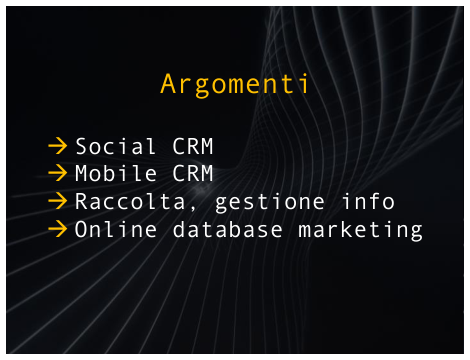
\includegraphics[width=0.50\textwidth,
                    trim=40 100 40 60, % L B R T
                    clip]
                    {images/Lez09_p01_fig_02}
  % \caption{Sommario}
  % \label{fig:Lez15_p06_fig_02}
\end{figure}
\FloatBarrier
\noindent

\section{Customer Relationship Management 2.0 - CRM 2.0}

Ma due parole sul titolo Customer Relationship Management 2.0.

Evidentemente una locuzione adottata dalla seconda generazione del web, web 2.0, caratterizzata dalle tecnologie, dai modi, dall'atteggiamento comunicativo sociale.
Infatti è stata donata al Customer Relationship Management questa nominazione generazionale 2.0 perché come vedremo ha seguito una evoluzione verso un maggiore rapporto sociale con il cliente anche a seguito della spinta successiva causata dalla forza mobile, quindi l'arrivo, l'adozione di tutte le tecnologie mobile sia da una parte cellulari e tablet, sia anche tutti i device magnetici che vengono utilizzati per fornire informazioni e per etichettare gli oggetti.

\subsection{Social CRM}

\FloatBarrier
\begin{figure}[H]
  \centering
  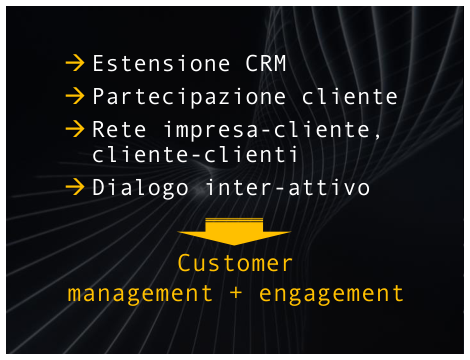
\includegraphics[width=0.50\textwidth,
                    trim=40 40 40 40, % L B R T
                    clip]
                    {images/Lez09_p01_fig_04}
  % \caption{Sommario}
  % \label{fig:Lez15_p06_fig_02}
\end{figure}
\FloatBarrier
\noindent

Social Customer Relationship Management è una estensione del Customer Relationship Management che porta ad una maggiore partecipazione del cliente e contemporaneamente la maggiore partecipazione è richiesta dall'atteggiamento del nuovo atteggiamento dell'azienda customer centred piuttosto che product centred, quindi focalizzato più sulla esigenza, sulla necessità, sulla soddisfazione del cliente, sul parere del cliente piuttosto che non sulla elaborazione e valutazione del prodotto.

Viene estesa la rete, consideriamo la rete dell'impresa con l'inserimento del cliente o delle comunità clienti e la costituzione di reti che coinvolgano clienti, quindi abbiamo l'azienda, l'organizzazione che si estende e apre la propria rete relazionale verso i clienti, e partecipa allo sviluppo di altre reti, peraltro spontaneamente costituite a volte, di comunità di clienti.
Il dialogo è interattivo, il Social Customer Relationship Management poggia sul dialogo interattivo, il termine interattivo fa riferimento alla partecipazione, allo svolgimento di un'attività in maniera partecipata da più attori, quindi da comunità di attori.
Questo ha portato a una estensione di quello che era il customer management con un nuovo elemento customer engagement, cioè non è più solo di interesse per l'impresa, la gestione del cliente quale consumatore, ma diventa importante il suo engagement, quindi la ricerca dei clienti, la fidelizzazione dei clienti, il seguire il cliente, avere una relazione permanente e continuativa con i clienti.
Due fattori hanno influenzato notevolmente questo fenomeno, lo user generated content e il social media.
User generated content fa riferimento ai contenuti, alle informazioni che vengono prodotte dagli utenti e il social media ai nuovi canali che permettono a quantità di attori di scambiare messaggi, mandare informazioni, di comunicare.
In quest'ambito i clienti o a fronte di questa spinta i clienti diventano editori, quindi produttori dei loro pareri, produttori dei feedback, quindi di messaggi da mandare alle aziende.
Non sono più solo le aziende che mandano bollettini, mandano descrizioni di prodotti, ma gli utenti diventano veri e propri editori di informazioni riguardanti prodotti.
Le imprese entrano nella rete sociale, le imprese entrano nella rete sociale perché?
Le imprese entrano nella rete sociale per partecipare alle conversazioni con i clienti, avere un diretto riscontro dei loro pareri, poter controllare i loro desideri, controllare nel senso di venirne a conoscenza nell'immediato, poter reagire dialetticamente nell'immediato, ma poter anche intervenire nel ciclo produttivo con modifiche rapide, modifiche tempestive.
I clienti diventano clienti sociali, gli acquisti vengono effettuati su opinioni, basandosi anche su opinioni o giudizi di altri clienti.
In effetti i prodotti vengono promossi e effettivamente o in maniera complementare alla pubblicità dagli stessi clienti sociali che presentano le loro esigenze, le loro ricerche di prodotti e contemporaneamente o diciamo allo stesso modo in un tempo successivo naturalmente propongono i loro o comunicano i loro feedback, i loro pareri, il loro livello di soddisfazione.
Questo ha reso il cliente utente, il cliente non è più il consumatore passivo di un prodotto, il consumatore di un prodotto che può essere soddisfatto o insoddisfatto e manifestare in maniera diretta con eventualmente il cambio di produttore, il cambio di prodotto, il non consumare più quel prodotto, ma comunica il proprio parere, partecipa da suggerimenti, partecipa alla modifica del prodotto stesso.
In quest'ambito sociale l'outcome based community è stata ideata per il coinvolgimento dei clienti dalle organizzazioni, sono comunità che coinvolgono i clienti e sono orientate a raggiungimento di obiettivi, di interesse per l'organizzazione.
Quindi il primo punto è il coinvolgimento dei clienti, poi la comproduzione dei prodotti e dei servizi, cioè i clienti vengono coinvolti come utenti per essere coinvolti nella gestione del ciclo produttivo dei prodotti o nella gestione dei nella buona conduzione dei servizi.
I prodotti usati sono effettivamente scelti dagli utenti, non sono adottati perché sono diventati status symbol piuttosto che indotti dalla pubblicità, piuttosto che prodotti alla moda, ma sono scelti più consapevolmente dai clienti.
Le aziende possono acquisire nuove idee a basso costo, prodotte fornite proprio dagli utenti che sono stati coinvolti in questo circuito, che sono stati coinvolti nel ciclo di vita del prodotto dalle organizzazioni.
Questa quantità di interazioni sociali produce naturalmente una gran quantità di informazioni che vengono inviate, vengono scambiate, che inducono la necessità di integrazione di dati, di valutazione delle fonti, parleremo web reputation, e di analisi delle sensazioni rappresentate in quei individuabili, in questi messaggi che sono analizzati in quella che chiamiamo e che vedremo sentiment analysis.
L'integrazione dei dati.
Da una parte i dati sono acquisiti dai social media o direttamente oppure analizzando i messaggi scambiati nelle comunicazioni delle community network.
E dall'altra parte questi dati vengono integrati con quelli gestiti dal back office dell'organizzazione e organizzati in quelli che sono data warehouse, cioè organizzazioni tematiche di dati sorrette da archivi eterogenei e archivi distribuiti, gestiti però dalla organizzazione.
La web reputation.
La web reputation fa riferimento all'attendibilità di una fonte e quindi la sua rispettabilità, la validità, la correttezza delle informazioni che nel tempo sono state trasmesse.
Ricordiamo che non facciamo solo riferimento ad archivi permanenti di informazioni che sono già state filtrate e analizzate, ma a informazioni che possono essere tratte o da pagine web estemporane o anche da discussioni del tutto informali in rete.
La pertinenza.
Le informazioni devono essere anche riguardanti l'argomento.
Il dato che viene trasmesso, che viene estratto, dovrà essere rilevante per l'argomento che si sta trattando o per il contenuto che si sta costruendo con la raccolta di questi dati.
Il terzo punto è l'importanza.
L'importanza sia in termini di rilevanza per chi le recupera, ma anche in termini oggettivi di importanza per quanto riguarda il problema informativo che si sta affrontando in quel momento.
La sentiment analysis fa uso dell'analisi del linguaggio naturale natural language processing, della linguistica computazionale degli strumenti offerti dalla linguistica computazionale e dalla analisi dei testi.
Per analizzare, elaborare i messaggi, le informazioni ricevute dagli utenti o scambiate tra di loro e evidenziare, estrarre pareri, sentimenti, quindi soddisfazione o manifestazioni di non gradimento di un servizio o di un prodotto sulla base di termini qualitativi, piuttosto che di frasi, piuttosto che adesso di simboli o emoticon a riguardo.
Alla fine di questo argomento vorrei ora proporvi uno spunto di riflessione.
Provate a fissare un prodotto, un'azienda e un target customer, quindi un un utente bersaglio, e immaginare ed descrivere il tipo di flusso di informazioni che può fluire tra di loro.
Passiamo ora all'argomento successivo, il mobile customer relationship management.
È una strategia di customer relationship management che utilizza tecnologie multicanale per la comunicazione, per la pubblicazione, la diffusione delle informazioni.
Serve d'aiuto sia ai dipendenti fuori sede, quindi ai commercianti, ma anche per il contatto ubicuo col cliente.
Contatto ubicuo, cioè per contattare il cliente dovunque si trovi e in qualunque momento possiamo raggiungerlo.
Per una definizione del mobile customer relationship management, il mobile marketing association, che è un'organizzazione, un'associazione di categoria no profit fondata nel 2000, con sede negli Stati Uniti a New York che coinvolge più di 700 società differenti in 50 paesi.
A sedi nel Nord America, in Europa, in Africa, nel Medio Oriente e in Asia.
Ha prodotto, ha proposto una definizione del mobile customer relationship management.
Come utilizzo strumenti wireless, veicolo per il trasferimento di contenuti e per fornire una risposta diretta all'utente in un ambito di comunicazione integrato.
E vorrei porre l'accento su tre termini particolari in particolare di questa definizione.
Wireless, risposta diretta dall'utente e comunicazione integrata, che ci ricordano la possibilità di essere raggiunti dovunque, senza necessità di un nostro volontario collegamento, per ottenere delle risposte immediate dall'utente per fornire informazioni, novità, pure nell'immediato, istantaneamente nel momento della loro produzione e attraverso strumenti di comunicazione integrati.
C'è una tale varietà per cui devono essere scelti, selezionati, utilizzati sulla base delle necessità di quel target di clienti.
I benefici portati sono che è raggiungibile, è interrogabile, si può comunicare col cliente in movimento dovunque si trovi, istantaneamente, in maniera persistente, fino a che l'utente possiederà il device di comunicazione, è possibile raccogliere dati contestuali utilizzando per esempio le tecnologie di geolocalizzazione o di prossimità digitale, quindi andando a cogliere il device non tanto interrogando il cliente per localizzarlo, capire in che area si trovi.
In questo caso, di norma viene chiesta l'accettazione da parte del cliente per essere localizzato o per accettare questo frequente scambio di informazioni.
Vi sono diversi tipi di approccio al mobile, quindi di tipi di scambio di messaggi, l'SMS, l'MMS o gli app, che sono gli applicativi utilizzati dagli smartphone per utilizzare servizi più complessi.
Vengono utilizzati come abbiamo accennato a prossimità digitale, quindi l'utente si approccia con un device trasmittente o ricevente, ha un device per la raccolta delle informazioni e viene agganciato, diciamo, viene rilevato il device che porta e quindi può iniziare la comunicazione.
Vi sono anche servizi di geolocalizzazione che fanno uso del satellite per individuare dei telefoni mobili autorizzati ovviamente dall'intestatario e fornire le coordinate geografiche a un sistema di gestione dei dati territoriali che potrà fornirli eventualmente mediante tecnologia web service a un meccanismo, a un'applicazione per la contestualizzazione di questi dati.
Alla fine di questo argomento vorrei proporvi come al solito uno spunto di riflessione.
Lo spunto di riflessione consiste nella scelta da parte vostra di un prodotto e di un target consumer e la descrizione di approcci di comunicazione e situazioni, contesti d'uso.
Passiamo ora al successivo argomento, la raccolta e la gestione di informazioni.
L'attività primaria in quest'ambito è il database marketing dedicato alla raccolta e l'analisi di dati per la rilevazione, per procurare clienti potenziali o per comunicare con clienti attuali, per la fidalizzazione o per lo scambio, per il loro coinvolgimento come abbiamo visto nel ciclo di produzione.
Il customer relationship management system interagisce o supporta meglio questa attività con i suoi tre elementi collaborativo e operativo con il customer service e support e con il livello analitico.
Ricordo che il livello collaborativo e il livello che opera mediante il front office e si dedica primariamente alla raccolta delle informazioni dal client, quindi dalla parte esterna, dall'estensione esterna dell'organizzazione.
Il livello operativo o di customer service e support produce e utilizza sintesi per operazioni di marketing e il livello analitico è quello che si occupa dell'archiviazione, dell'organizzazione, della produzione delle sintesi di base dei dati, la pulizia dei dati e la loro organizzazione.
I dati sono eterogenei, c'è una grande quantità di dati eterogenei e vengono quindi organizzati in data warehouse.
Non è possibile con questa varietà di dati supporre una gestione omogenea dei dati, omogenea per quanto riguarda il sistema adottato.
I data warehouse allora sono dei sistemi che permettono l'organizzazione tematica dei dati a seconda di argomenti o a seconda di una loro omogeneità di pertinenza.
I dati rilevati dai clienti vengono quindi archiviati, elaborati per creare, produrre nuove prospettive aziendali.
Vi sono due fonti di dati che primariamente consideriamo, i dati primari e i dati secondari, i dati primari sono dati che forniscono un parere diretto sui prodotti e sui servizi.
Vengono prodotti dall'azienda attraverso esperimenti o indagini, indagini attraverso questionari inviati ai clienti, agli utenti o proposti in comunità online o esperimenti che possono essere effettuati con contatto diretto, con coinvolgimento personale diretto dei clienti.
La gestione, l'acquisizione di questi dati è impegnativa, costosa ma è necessaria perché sono i dati diretti sui prodotti ma soprattutto perché la fonte è ovviamente apprezzabile dall'organizzazione perché sono prodotti dalla organizzazione stessa.
Vediamo ora i dati secondari.
Sono una base per dedurre dati diretti sui prodotti, sono dati disponibili ed eventualmente pubblicati.
I dati possono essere interni, provenire quindi dalle vendite, dai feedback raccolti dagli utenti, da comunicazioni avvenute con loro o da operazioni di marketing.
Oppure possono essere esterni, ottenuti da pubblicazioni, da ordini d'acquisto o da internet, quindi dalla consultazione dei siti di presentazione di questi prodotti oppure dai siti per l'acquisto o semplicemente da altri comportamenti, da altre navigazioni dell'utente che è registrato o conosciuto dall'organizzazione, dall'impresa.
I dati sono categorizzati tematicamente sulla base dei dati di identificazione quindi indirizzo, numero di telefono, dati anagrafici che riguardano il cliente.
Eventualmente, naturalmente, l'indirizzo di IP per internet o il numero di cellulare o le coordinate del suo cellulare se già localizzate.
I dati demographici quindi lo studio, il reddito, ma per reddito anche più limitatamente il tipo e la quantità di spesa effettuata in che settore commerciale gli interessi le sue abitudini.
I dati psicografici o dello stile di vita che riguardano i valori dati dai clienti ai prodotti, le proprie preferenze, le attitudini e così via.
I dati transazionali che non possono essere procurati da fonti esterne ma si riferiscono ai dati effettuati con gli scambi acquisti o resi con il produttore o con il fornitore.
Infine i dati di marketing che dipendono o sono prodotti dalle tattiche strategie intraprese dall'azienda.
Alla fine di questo ulteriore argomento vorrei proporvi un ulteriore spunto di riflessione.
Scegliete un prodotto e un target customer e individuate le informazioni per fonte e categoria tematica.
Passiamo ora al successivo argomento online database marketing.
E' svolto con diverse attività rilevanti quali la web analytics innanzitutto che si occupa della raccolta dei dati online, l'attributo web si riferisce sia alla navigazione effettiva di pagine web ma ora anche all'accesso ad archivi, consultazioni di informazioni piuttosto che non l'analisi di conversazioni effettuate in social community.
Diciamo che sarebbe più corretta una locuzione internet analytics, riferendosi a tutti i servizi che sono frequentati dal utente e non solo quello ipertestuale.
Infatti ci riferiamo alla raccolta di dati online, alla loro misurazione, eventualmente per la frequenza, la clusterizzazione, la selezione delle attività svolte dall'utente, in questo caso attività che possono essere primarie di navigazione, l'azione su un'ancora, piuttosto che l'accesso di una pagina, piuttosto che la consultazione di un documento che possono essere trascurate o raggruppate per capire il tipo di sessione, il tipo di uso, di consultazione che il cliente sta facendo in quel momento del servizio online.
I dati vengono quindi analizzati per raccolti organizzati in profili di utente in genere, per produrre rapporti che ci facciano capire, ottimizzare il comportamento commerciale degli utenti.
Ma un'attività basilare per questa reportistica o per capire effettivamente il comportamento degli utenti è la profilazione, la profilazione online, cioè l'attività che ci permette di avere una completa visione dell'utente attraverso dati che riguardino il lavoro, l'istruzione, gli hobby, quindi i passatempi, i suoi interessi, i tipi di navigazione ed acquisti.
Ma questo tipo di dati che può essere acquisito attraverso l'osservazione del cliente vengono integrati con le sue conversazioni, gli acquisti effettuati e le interazioni sia attraverso le application con gli smartphone eventualmente, sia attraverso l'analisi dei dati di navigazione ma anche riguardanti direttamente gli acquisti fatti in presenza online, la frequenza delle sue azioni e via.
Queste informazioni sono integrate con ulteriori riguardanti gli interessi diretti o attraverso friend over friend, un metodo di analisi dell'interesse o delle similitudini, delle empatie di persone in rete con altre persone, quindi gli scambi proposti o allacciati con persone naviganti in rete che hanno interessi analoghi e quindi possono fornire informazioni indirette sul nostro cliente.
Ma come funziona il processo per la costruzione di un profilo di utente?
Innanzitutto va creata una identità online, da una registrazione quindi l'utente consapevolmente decide di fornire le proprie informazioni, nome, cognome esplicitamente si rappresenta, si descrive come vuole lui stesso, oppure in mancanza di questo viene utilizzato dal sistema di raccolta informazioni l'indirizzo IP, è sempre posseduto da chi naviga, da qualsiasi device collegato in rete internet.
Questo inizio di identità viene arricchito con la tracciatura di tutte le informazioni, di tutte le azioni che vengono svolte da questa identità.
Queste informazioni devono essere poi ovviamente ripulite, analizzate, raggruppate, sintetizzate, integrate per costruire delle informazioni rilevanti di interesse per l'analizzatore, per l'enterprise.
Vi sono due tipi di raccolta di dati, reattiva, il cliente è consapevole, questo tipo di raccolta di informazioni deve essere utilizzata per la raccolta di informazioni delicati, informazioni che possono riguardare la privacy, informazioni che per essere raccolte implicano una entrata in un'attività personale del cliente, oppure dall'altra parte raccolta non reattiva, il cliente è inconsapevole.
In questo caso possiamo far riferimento a informazioni anche se è un'inconsapevolezza un po' leggera, la cattura delle informazioni durante la navigazione dell'utente.
Dico che è un'inconsapevolezza leggera nel senso che tutte le operazioni effettuate in rete vengono memorizzate dai server, vengono archiviate per questioni di sicurezza, questioni di protezione della privacy, questioni di individuazione di accessi scorretti, ma anche naturalmente per positivamente produrre o contribuire a questa analisi dei comportamenti che possono riguardare il sito specifico o dall'altra parte come in questo caso stiamo vedendo, web analytics, quindi profili di utente.
Vi sono due tecniche di raccolta dei dati, una è accessi al server, come dicevo tutte le operazioni svolte da un navigante in rete, tutte le operazioni svolte in rete su un'applicazione in rete vengono memorizzate in un file, vengono archiviate dal server che gestisce, che offre l'applicazione.
L'altra tecnica è attraverso i page tag, vediamo nell'ordine, l'analisi degli accessi al server viene fatta archiviandoli in un access log file che è un archivio che contiene l'indirizzo IP dell'utente, l'indirizzo IP che è posseduto sicuramente dal device per interagire che sta usando in quel momento l'utente e può essere utilizzato anche come identificativo in prima istanza dell'utente stesso.
L'access log file può contenere anche un identificativo di utente in caso di registrazione o in caso di accesso protetto, quindi di login.
L'access log file registra pure la data e l'ora dell'azione dell'utente, un click su un'ancora, l'accesso a una pagina, una scelta, un'operazione di acquisto, una consultazione, l'apertura di un file di catalogo o l'ingrandimento di un prodotto proposta in quel dato istante.
Viene archiviato anche il codice dell'esito dell'operazione, quindi se l'operazione dell'utente è stata effettuata con successo oppure no.
Il volume della risposta, questa è un'informazione tecnica non molto utile, presumo per la definizione del profilo, ma diciamo che il log file archivia anche il traffico di informazioni che è stato effettuato dalle operazioni richieste dal cliente durante la sua navigazione.
E l'agente che è una riga descrittiva del sistema operativo utilizzato dall'utente.
L'altra tecnica è quella dei page tag, chiamata page tag.
Sono istruzioni in JavaScript sorgente inseriti nella pagina web per misurare l'interazione dell'utente, per catturare il tipo di operazione effettuata dall'utente interagendo con la pagina, per controllare questo tipo di attività e per conteggiare o le operazioni, gli accessi alla pagina o in qualche modo le interazioni effettuate.
A questo punto l'argomento è completato e vi propongo in conclusione uno spunto di riflessione.
Definire un profilo di utente sulla base di quanto visto ed descrivere la provenienza e metodo di acquisizione di ogni attributo che avete inserito.
Vi ringrazio per l'attenzione, vi ricordo che sul portale dell'Università Telematica Uninetuno troverete a disposizione materiale documentale di approfondimento e una bibliografia.
Arrivederci.